\chapter{Website}
\section{Features}
In this project, the only objective of the website was to collect information from the user, and stock them in the database.

When an user comes for the first time on the website, he has to sign up and provides some informations about the company. After this operation, the user can access to his control panel where he can:
\begin{itemize}  
\item Create or edit his switchboards.
\item Manage operators\footnotemark.
\item Manage the company's informations
\end{itemize}  


\footnotetext{Operators are people who will receive calls from the switchboard.}

\section{Available modules}

\subsubsection{Playback}

\subsubsection{Operator}

\subsubsection{Queue}
\subsubsection{User input}



\section{Overview}
In this project, the website had to be the only way to interact with the server. Through a simplified website, the users have to fill required informations, then they are saved into a database.
\newline

The website is based on \textbf{Spring} technology,  it follows the MVC convention (\textit{Model-View-Controller}). Each layer has its own role in this convention.


\begin{itemize}  
\item The views represents the content the users will be able to see. In our implementation, these files contains special HTML and special tags to allow dynamic contents. 
\item The controllers corresponds to global files 
\item The model represents the database data. It will perform SQL queries to get some data in order to return them as a simplified object to a controller.
\end{itemize}  

Here is a schematic representation of the website architecture

\begin{figure}[!ht]
  \caption{MVC.}
  \centering
    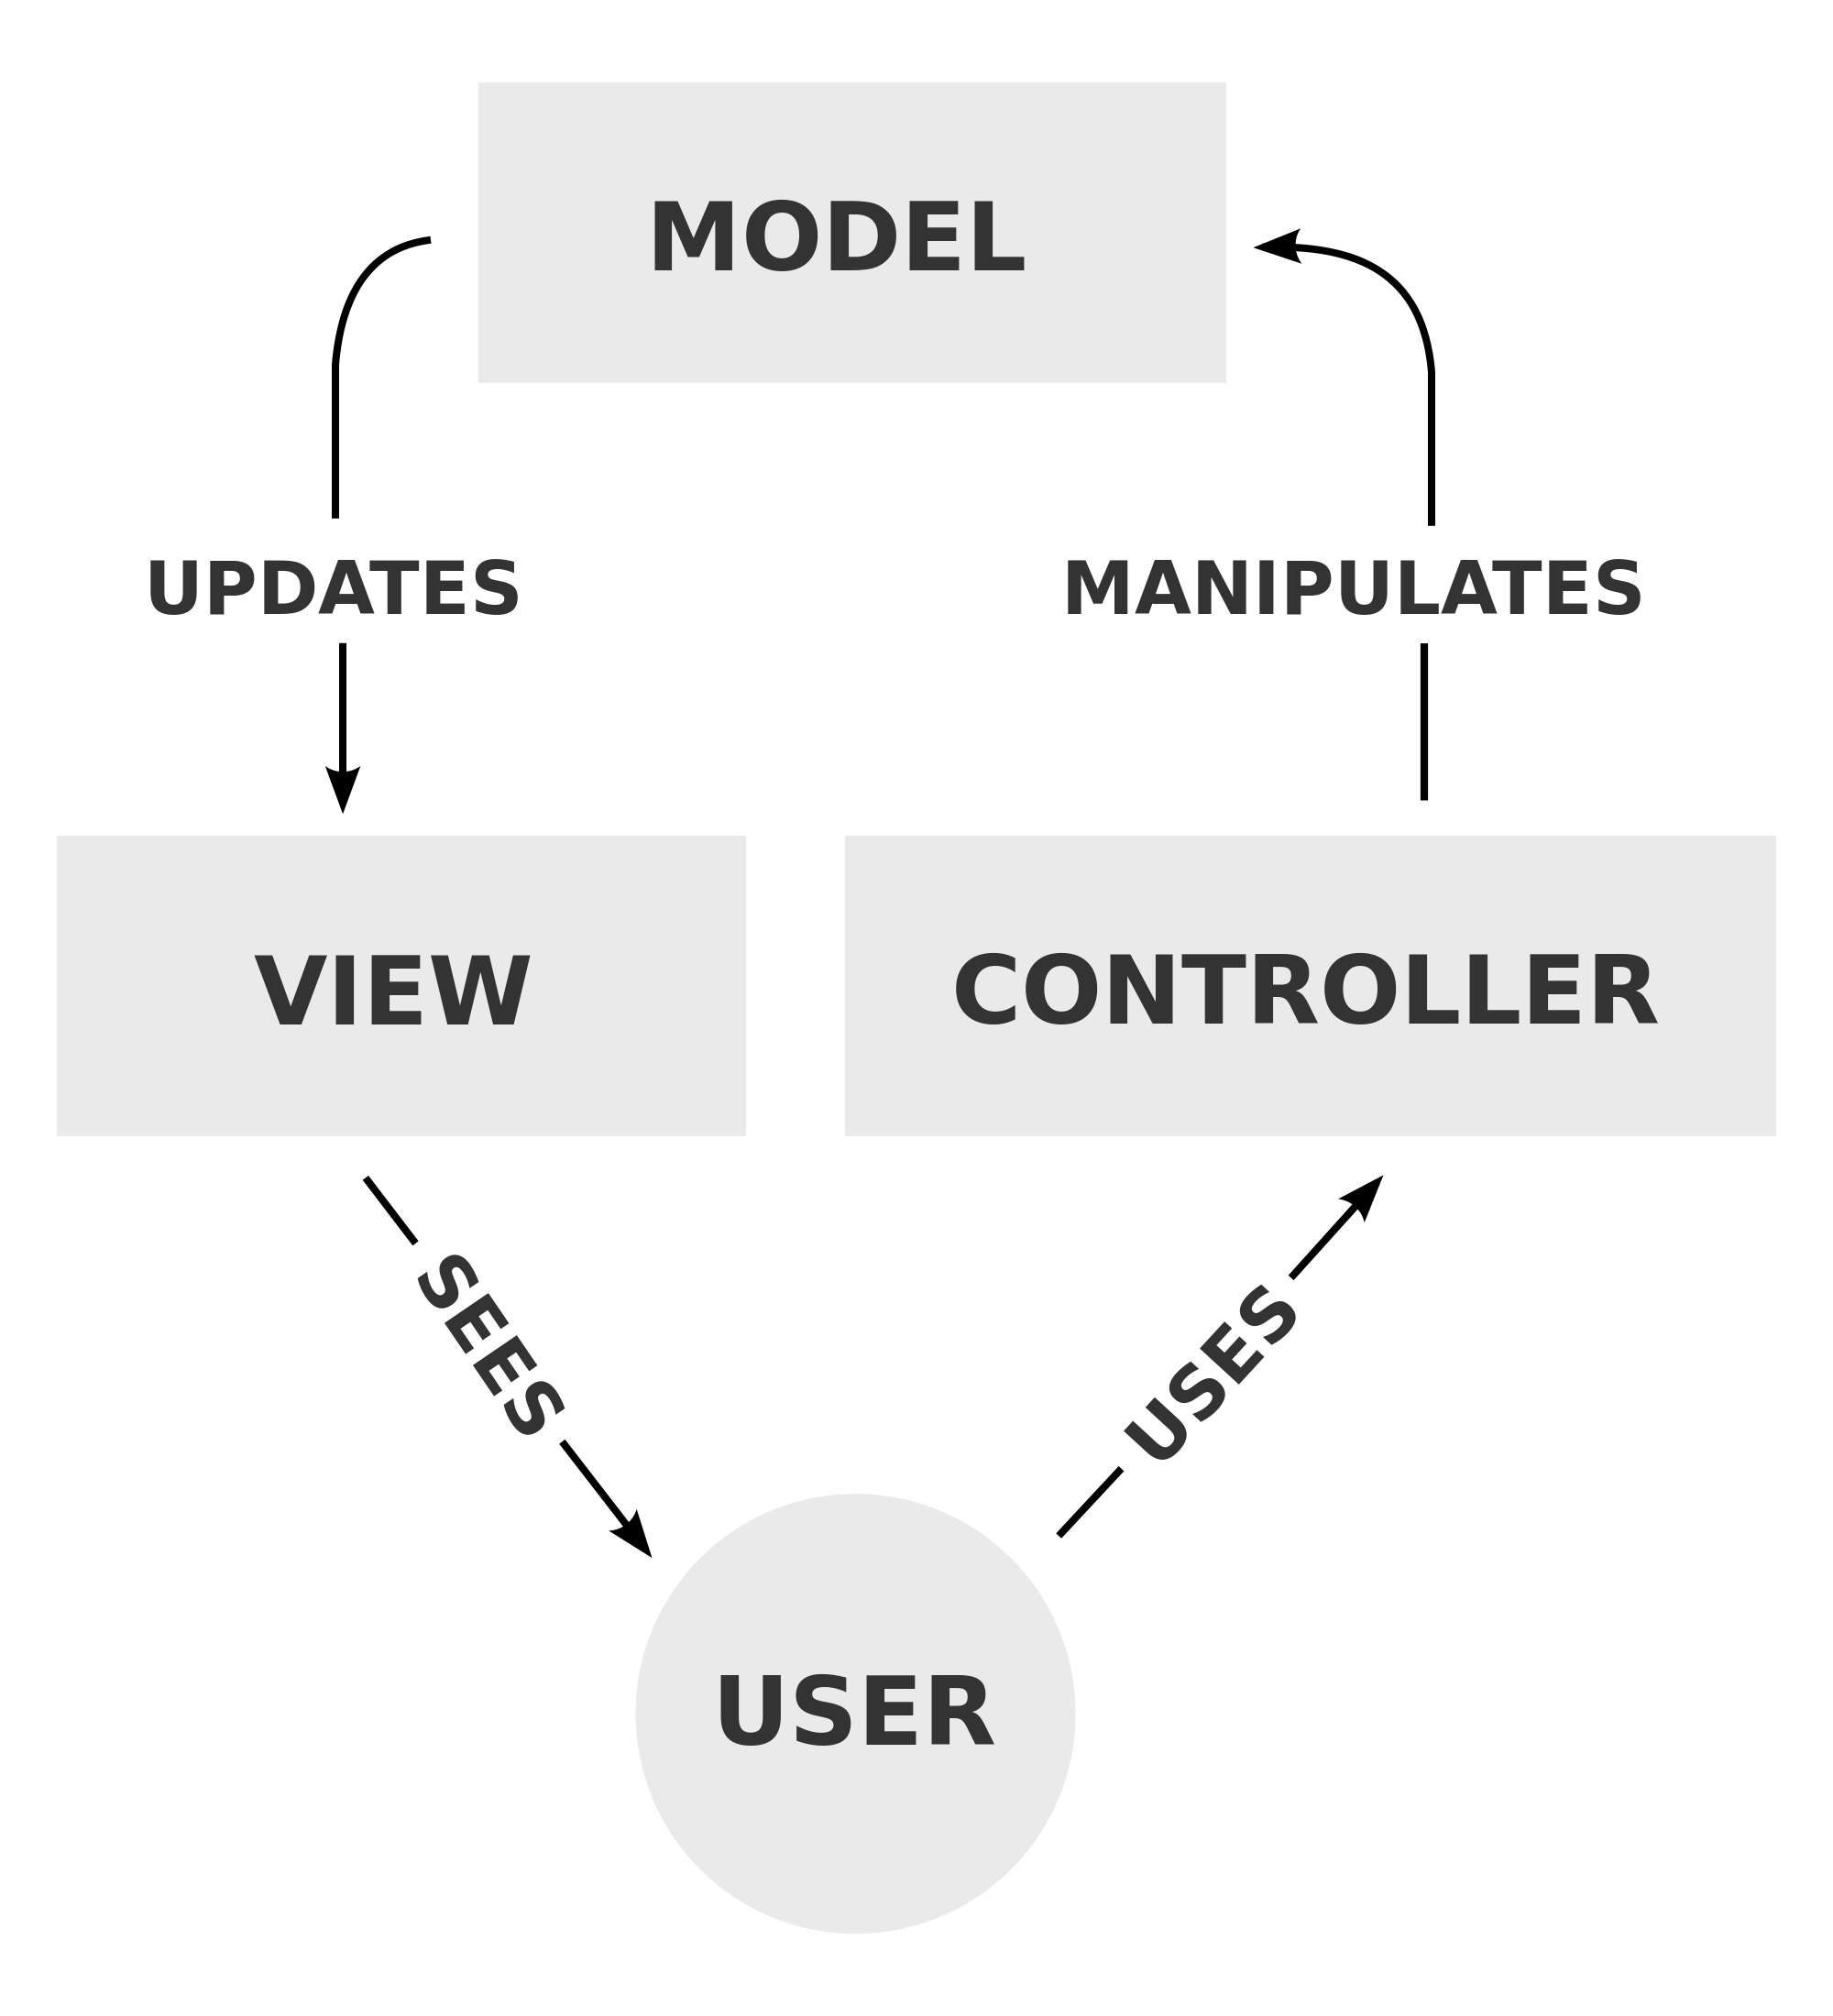
\includegraphics[width=0.5\textwidth]{img/mvc.png}
\end{figure}

\newpage

\section{Spring application}
\subsection{Why Spring instead traditional J2EE?}

\begin{figure}[H]
  \caption{Logo Spring.}
  \centering
    
\includegraphics[width=0.2\textwidth]{img/spring.png}
\end{figure}


Spring is the most popular JAVA framework, It is used in a large parts of professional projects due to its stability, performance and security.
It have a lot of features such as:

\begin{itemize}  
\item Spring provides an easy and secure way to handle forms. With help of DTO for validation, everything is almost automatic.

\item Spring manages the instantiation of the objects without developer worrying about placing instances, when Spring create only one instance and successive calls returns the same object by use of \textit{@Autowired} annotation.

\item Spring is developed in its core with design pattern as Singleton, Factory, MVC... and it is why it is so powerful.
\item Spring is able to manage the dependencies and the configuration of others frameworks.
\end{itemize}  



\subsection{Annotations...}

With Spring and Hibernate, annotations have a very important place in our code, it helps the framework to understand the code and apply special action according to these annotations.
An annotation always begin with the character \textbf{@} and it is placed above a class, a method or an attribute.

\subsubsection{@Autowired and injections}
@Autowired is a Spring specific annotation, It signal to the framework that it have to inject something special at this location.

\begin{figure}[!ht]
  \caption{@Autowired example}
  \centering
    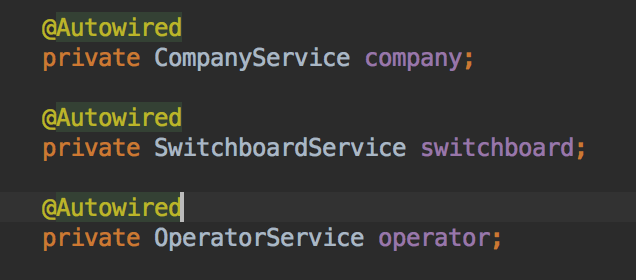
\includegraphics[width=0.7\textwidth]{img/autowired.png}
\end{figure}

In this example, Spring will automatically find the 3 class corresponding to these declarations, and will automatically inject an object and will stock it in cache. So if we call it after again, we will gain performance because it will not be created again.\newline

However, this example is not enough. When an \textit{@Autowired} request an interface, Spring will automatically find the best implementation of this interface.
 
\begin{lstlisting}[language=java,caption={JAVA}]
interface myInterface {}

class MyImplementation implements myInterface {}

public class MainClass {

	// Contains an object of class: MyImplementation
	@Autowired
	private myInterface myObject; 
}
\end{lstlisting}




\section{Application structure}

\subsection{Configuration}
To properly use Spring, we have to let it know which kind of application will be created. Indeed, Spring is a really powerful framework and can be used in lot of different usage.
The configuration of Spring is mainly made by usage of annotations and implementations of some \textit{interfaces}. All following class have to be annotated with \textbf{@Configuration}.\newline

Firstly, we have to tell Spring the application will be a website. According to the official documentation, we have to create a class called \textbf{SpringMvcInitializer} which implements \textit{WebApplicationInitializer}.\newline

Now, Spring knows it will run a website. However, we have to configure some things before it can work properly. We have to create a class \textbf{WebMvcConfig} which extends \textit{WebMvcConfigurerAdapter}. It is in this file, the main settings will be made. For example, it is here we can define the \textbf{view resolver} (we chose Pebble), which will make Spring able to load the views files.  Some others settings will be described in next sections.
\newline


\subsection{Login mechanism}

\begin{figure}[H]
  \caption{Login schematic}
  \centering
    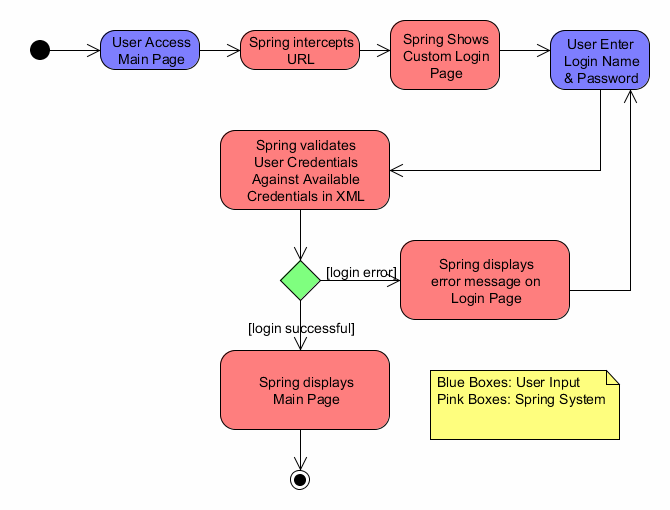
\includegraphics[width=1\textwidth]{img/login.png}
\end{figure}


Here is a schematic representation of a login request processed by Spring, the framework is delivered with its own authentication method in its core. It is why we used this inbuilt system to make our login system. However, its default behaviour doesn't match our requirements. Indeed, by default the login has to be made with an username and a password while we would like to use an email authentication. 

\begin{figure}[H]
  \caption{Login code.}
  \centering
    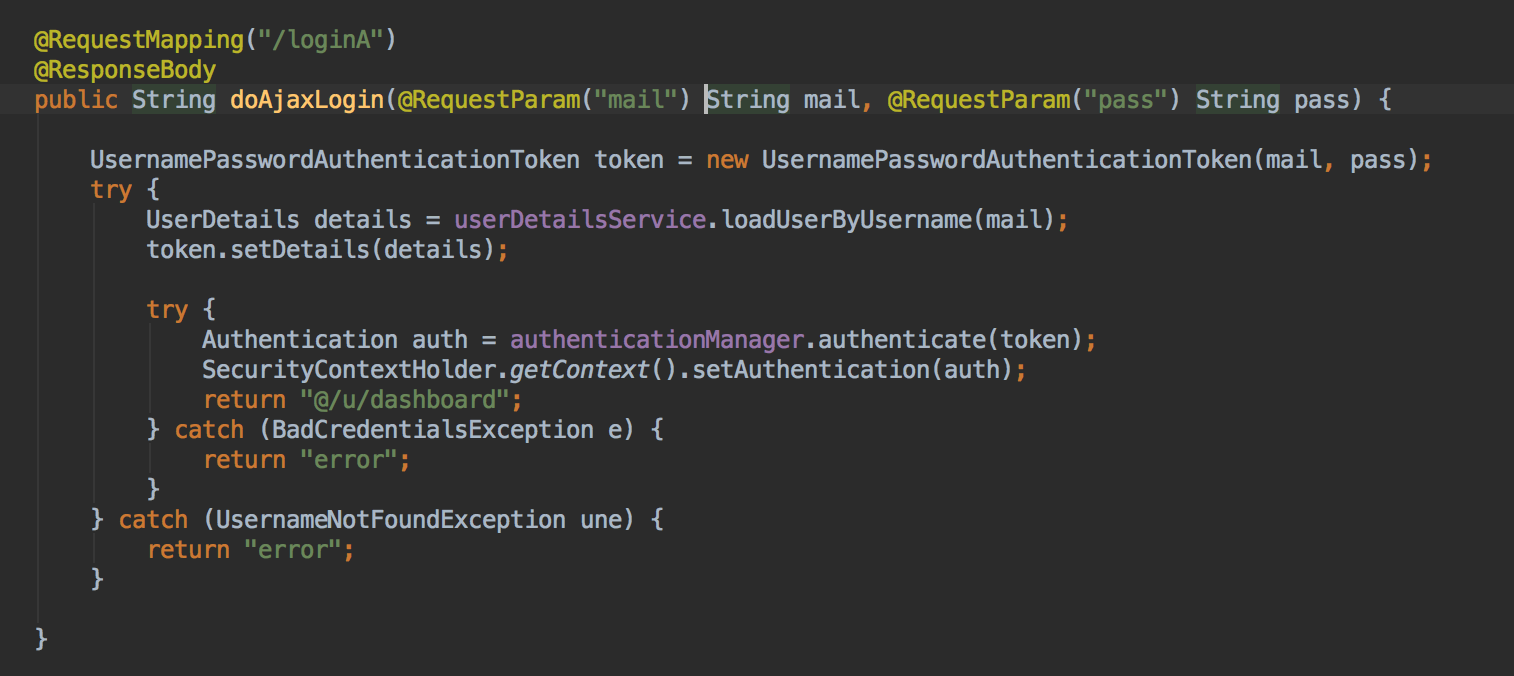
\includegraphics[width=1\textwidth]{img/loginCode.png}
\end{figure}

\subsubsection{User entity, Interface to implement}
To use this login mechanism, we had to implement the interface \textit{UserDetails}. 

\begin{figure}[H]
  \caption{UserDetails interface.}
  \centering
    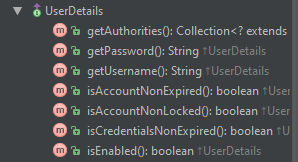
\includegraphics[width=0.7\textwidth]{img/userdetails.png}
\end{figure}

\subsubsection{User service}
As said before, the default behaviour doesn't match our needs. So, we have to create an \textit{UserServiceDetails} which implements the original service interface \textit{UserDetailsService}.

Inside, we have to redefine the method \textit{loadByUsername} to load an user by its email. 

\subsubsection{Security}
For this application, we chose to encrypt password for a better security. Because Spring checks itself if a password is right, we have to tell it how the password is encrypted. This can be done by extending the class \textbf{WebSecurityConfigurerAdapter} and customize the function \textit{configureGlobalSecurity(AuthenticationManagerBuilder auth)}.


\begin{figure}[H]
  \caption{Password encoder.}
  \centering
    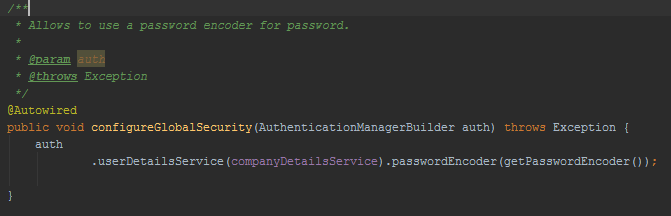
\includegraphics[width=1\textwidth]{img/passwordencoder.png}
\end{figure}




\section{Controllers}

The controllers are the link between the user and the kernel.
User ask for information : the controller transfer the request to the model, take informations and send them to the view
User give informations : the controller take these informations (after every verifications) and send them to the kernel


\section{Hibernate, a link to the Database}

Hibernate makes easier the interaction with the database where we don't have to use standard SQL interaction. 
Each traditional database table is represented by a JAVA class where all its fields are annotated. These class can also be linked to each other by some relations: \textit{ManyToMany}, \textit{OneToOne}, \textit{ManyToOne}...
All the database operations are made through an hibernate session which allows to read, create, update, delete...

\subsection{Configuration}
To use Hibernate with Spring, we had to configure it. As seen in a previous section, all the configuration can be done through a file annotated with the annotation \textit{@Configuration}. 
Because Hibernate uses the transaction system to save changes, have to use this annotation too: \textit{@EnableTransactionManagement}.


\begin{figure}[!ht]
  \caption{Transaction system.}
  \centering
    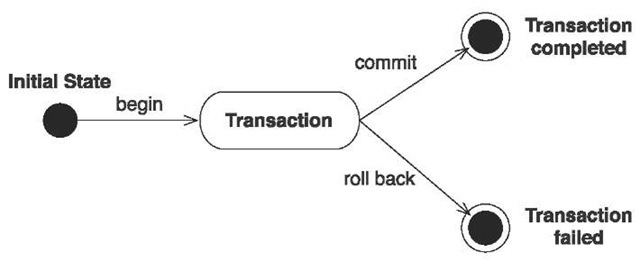
\includegraphics[width=0.7\textwidth]{img/transaction.jpg}
\end{figure}


Now, we have to tell Hibernate the correct settings to make it able to connect to the database:
\begin{itemize}
	\item \textbf{driver} - It corresponds to the JAVA driver to use. We used \textit{MySQL} as server: com.mysql.cj.jdbc.Driver
	\item \textbf{url} - It corresponds to the URI to connect to the database
	\item \textbf{username} - The login username
	\item \textbf{password} - The login password
	\item \textbf{dialect} - Because Hibernate can handle many SQL server, we have to tell it we will use a \textit{MySQL} server. 
\end{itemize}

\subsection{Entities annotation}
To describe the entities, once more we used Hibernate annotations. The following list contains all the annotations we used.

\begin{itemize}
\item \textbf{@Transient} - Prevent a field to be saved in database.
\item \textbf{@Column(name=...)} - Indicate the field has to be saved.
	
	\begin{itemize}
		\item \textit{name} - The name in the database, useful to fix these name and use them with the \textit{NodeJS} server.
	\end{itemize}
	
\item \textbf{@ManyToMany(fetch=...)}, \textbf{@JoinTable(name=..., joinColumns=..., inverseJoinColumns=...)} - Indicate a relation \textit{n,n}.
\begin{itemize}
\item \textit{fetch} - EAGER or LAZY mode. With EAGER mode, the relation will be loaded from database in same time that parent entity.
\item \textit{name} - The name in the database.
\end{itemize}

\item \textbf{@OneToMany(mappedBy=..., fetch=...)} - Indicate a relation of \textit{0,n}.
	\begin{itemize}
	\item \textit{mappedBy} - contains the name of the current entity in the remote entity
\end{itemize}


\item \textbf{@ManyToOne(fetch=...), @JoinColumn(name=...,nullable=...)} - Indicate a relation of \textit{n,1} with an other entity
	\begin{itemize}
	\item \textit{nullable} - tells Hibernate if the field can be null
\end{itemize}


\item \textbf{@ElementCollection(fetch=...)} - Save a \textit{List<?>} or \textit{HashMap<?,?>} object


\end{itemize}


\newpage
\subsection{Entities}

In this section, we will describe the entities we used in our project. 

\paragraph{Company:} 
This entity is used to represent a logged user. It contains some details about the \textit{company}, the password and one email.
 
\paragraph{Switchboard:}
This entity represents a company \textit{switchboard}. It contains global informations about this switchboard and contains \textit{modules}. 

\paragraph{Module:}
The \textit{Module} entity represents the application which will be used in dialplans. It contains all settings related to a \textit{module model}. 

\paragraph{ModuleModel:}
The \textit{module model} entity only contains an identifier for others server. This unique identifier 

\paragraph{Line:}
It represents the available phone numbers linked to the \textit{Asterisk} server. It contains the phone number, the region code and a boolean to indicate if it's a shared line. This entity is used by \textit{Switchboards} entities.

\paragraph{MOHGroup:}
This entity represents the playlist a caller will be able to hear. It only contains a name and a \textit{switchboard}.

\paragraph{MOHFile:}
This entity is associated at \textit{MOHGroup}. It represents a file in a \textit{MOHGroup}. It contains the filepath on the system and a name.

\paragraph{Queue:}
This entity represents the \textit{Queue} application and only contains a name and the name for \textit{Asterisk}. It is associated to a \textit{Switchboard}.

\paragraph{Operator:}
The \textit{Operator} entity is used to save the switchboard operators. It contains an username and a secret password if it is not a \textit{Skype} account.

\paragraph{SoundLibrary:}
This entity is only used to index the \textit{Asterisk} default files.

\paragraph{CallLog:}
This entity is useful to save some logs about the calls on the switchboards. It contains a caller number, a duration, a date... 

\begin{figure}[H]
  \caption{Entities relations.
  Full schema in Appendix section.}
  \centering
    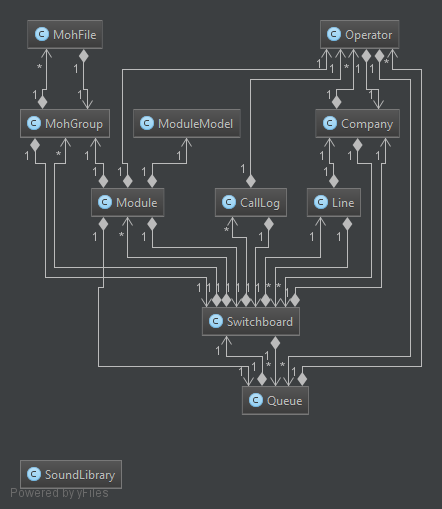
\includegraphics[width=0.7\textwidth]{img/modelsSimple.png}
\end{figure}




\subsection{DAO, repositories}


The DAO are the link between controllers, entities and the database. 
In fact, we have one DAO per entity (switchboard, company...), these files contains functions which returns informations from the database. 

In this way, controllers doesn't have to interact with database. It's the \textbf{M.V.C.} principle.

The DAO have to be defined as \textbf{interface}, then there have to be implemented.



\subsection{Converters}

Converters, as indicated by its name, can convert an object to an other one. Every converters have to implement the interface  \textbf{Converter<S, T>} . The method \textit{convert(S element)} have to return the new object formed with the first one. For example the converter \textit{OperatorIdToOperatorConverter} have for first element an Interger which represent the ID of an operator and it is returned the Operator corresponding. 

These converters are mostly used in the form process. For example, we can have a \textit{select} list which contains the operators name and the value attribute matches their id. To convert this integer value to an object in a DTO, Spring have to know how to convert it. The converters have to be registered in the configuration.

\begin{figure}[H]
  \caption{Converters code.}
  \centering
    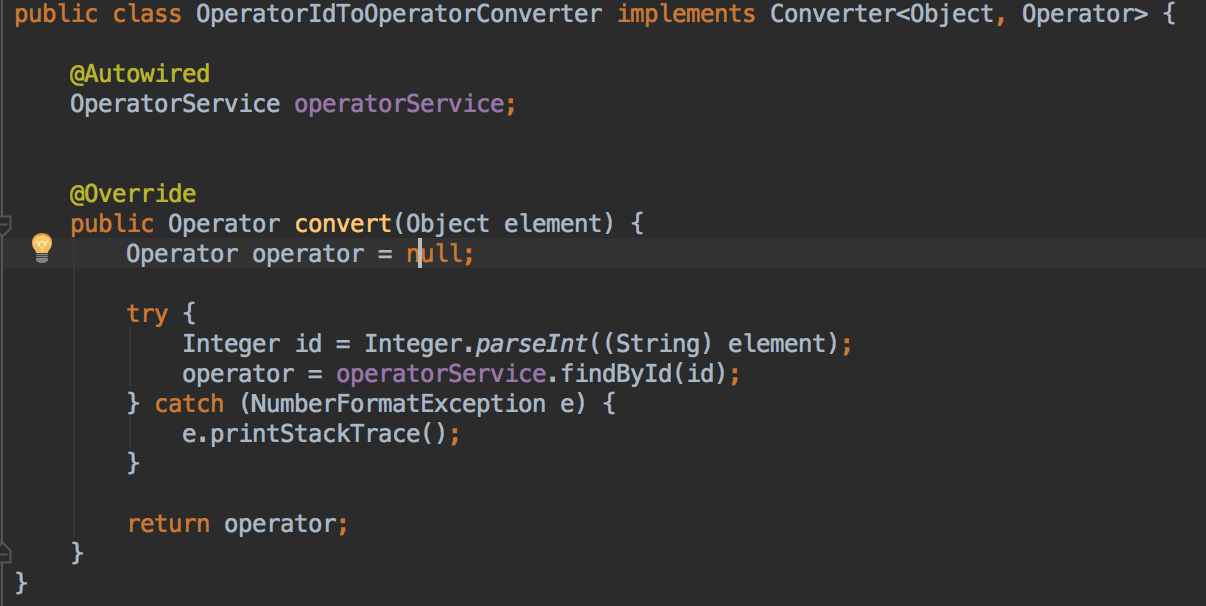
\includegraphics[width=0.8\textwidth]{img/converter.png}
\end{figure}



\subsection{DTO and Validator}

The DTO\footnotemark are a usually a copy of an entity, but it can also be the object representation of an HTML form. These DTO explain the entity constraints. For example we can say that one attribute should not be longer than 20 characters... 
When a form is submitted, the DTO fields will be automatically filled with the form fields, according to their matching names. 
\linebreak

When a DTO is used for a form, we can create a POST method in a controller. 


\begin{lstlisting}[language=java,caption={JAVA}]

public class MyEntityDTO {
	@Length(min=5, max = 10, message = "Your name should contains between 5 and 10 characters.")
	private String name;
	
	// getters, setter...
}

@Controller
public class MyController {

	@RequestMapping(value = "/myform", method = RequestMethod.POST)
	public String myPageProcess(MyEntityDTO dto, BindingResult result) {
		
		// check if form have some errors...
		if(result.hasErrors()){
			// process errors... 
		} else {
			// No error, can continue
		}		
		// ...
	}
}
\end{lstlisting}


\footnotetext{Data Transfer Object}


\section{Services}

We have an other types of files calls "Services", it works with the DAO files.
Their role are to check data sent from the application to the DAO, it prevents to avoid any error in the database.


\section{View}

The .twig files are an evolution of the HTML files, there are managed by pebble and represents the view of the website.
A .twig file can represent a file, or a part of a file (a layout), like a that we don't have to code every time the same code (like the menu...)
.twig offer something more than a classical html file, it allow to use Java object inside the view, so we can transfer a list and process it directly inside the view.



\subsection{Exceptions}

Exceptions are a special type of class which is call only when something goes wrong...
Java provide a large panel of exceptions, we can use them or create our own Exceptions.
The role of the excerptions are to identified quickly when an error occurred, we have a special name for every exceptions so we can know in a few seconds what is going wrong.


\section{Design}
Due to our inability to make a real design, we chose to download a free open-source design. We found the excellent \textit{AdminLTE2} template suitable for a website like our.
\newline

We cleared and adapted it to our website and needs.
This template is based on the Bootstrap framework which ease the front-end development of a website. Furthermore, the Bootstrap framework is a responsive design: it means our website will be functional on every platform (phone, tablets, computer...) and for all screens size.

\begin{figure}[!ht]
  \caption{AdminLTE2.}
  \centering
    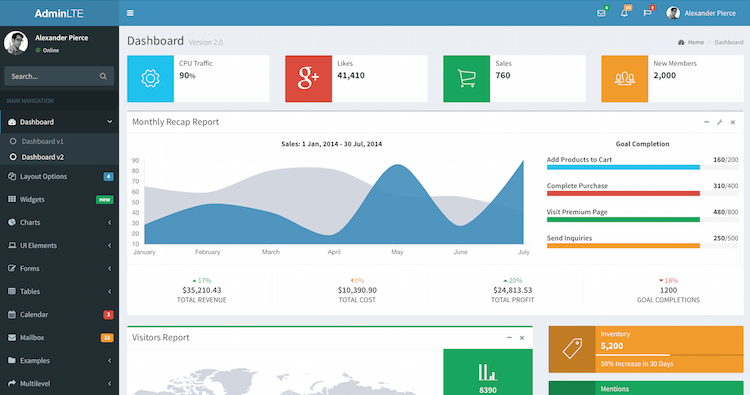
\includegraphics[width=0.9\textwidth]{img/design.png}
\end{figure}





